\setlength{\columnsep}{3pt}
\begin{flushleft}
\bigskip
\bigskip
\begin{figure}[h!]
	\centering
	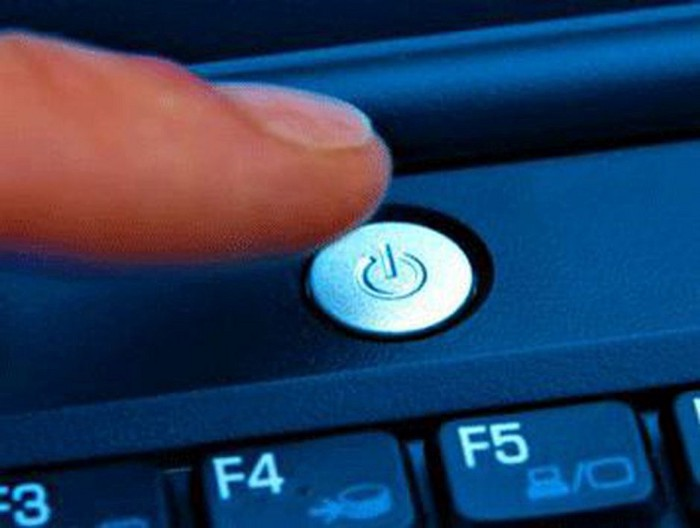
\includegraphics[scale=0.4]{content/chapter17/images/power_on.jpeg}
	\caption{Powering on PC}
	\label{fig:power}
\end{figure}


Step 1: BIOS
\begin{itemize}
	\item When you press the start button, the computer first reads a program called as \textbf{BIOS}.
	\item BIOS stands for \textbf{Basic Input Output System}.
	\item BIOS first performs \textbf{POST}.
	\item POST stands for \textbf{Power-On Self-Test}.
\end{itemize}
Step 2: POST
\begin{itemize}
	\item POST determine if the computer keyboard, RAM, disk drives, and other hardware are working correctly.
\end{itemize}
\newpage
Step 3: BIOS
\begin{itemize}
	\begin{figure}[h!]
		\centering
		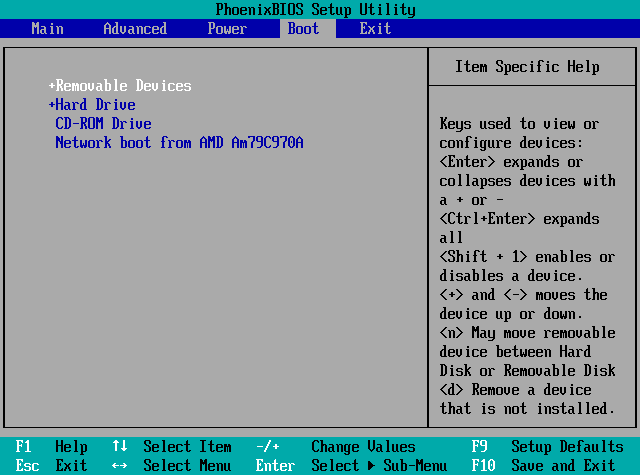
\includegraphics[scale=0.5]{content/chapter17/images/bos.png}
		\caption{BIOS}
		\label{fig:bios}
	\end{figure}
	
	
	\item Once the POST check is completed successfully, BIOS will look CMOS (stands for Complementary metal–oxide–semiconductor) settings to know what is the boot order:
	\begin{itemize}
		\item First preference is \textbf{Removable Device}.
		\item If it's not present, the bios will look at the second device from the boot order settings.
		\item The second device is your \textbf{hard disk}.
	\end{itemize}
	
\end{itemize}


\bigskip\bigskip
\begin{tcolorbox}[breakable,notitle,boxrule=-0pt,colback=yellow,colframe=yellow]
	\color{black}
	\textbf{Note:} By default, BIOS is not displayed during system startup. According to your hardware, you might have to press \textbf{F12} or \textbf{F10} or similar key combinations at the start of system boot to see the BIOS settings.
\end{tcolorbox}

\end{flushleft}
\newpage


